%\documentclass{article}
%\usepackage{graphicx,subfigure}
%\begin{document}

\begin{figure}[!h]
  \centering
   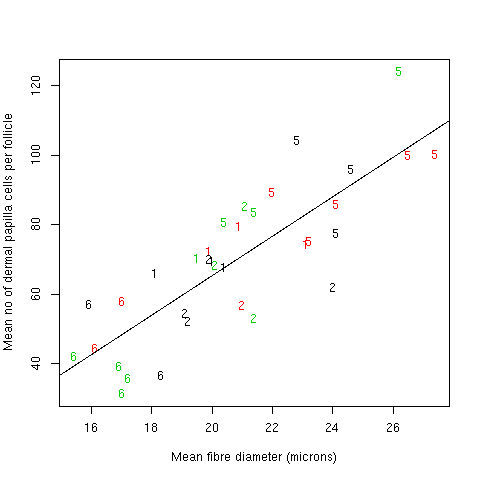
\includegraphics[width=0.9\textwidth]{dpccdiam.png}
  \caption{Plot of mean fibre diameter against mean number of dermal papilla cells per follicle for 34 sheep from CSIRO selection experiment AB46. The coloured numbers representing each point indicate the selection line (1 = high staple length, 2 = low staple length, 5 = high fibre diameter, 6 = low fibre diameter). The straight line is a  linear regression ( Y = -48.281 + 5.678 * X)  which had an $R^{2}$ of 0.672 ( corresponds to a correlation of 0.819) and the fit was highly significant.}
  \label{fig:dpccdiam}
\end{figure}

%\end{document}

